%!TEX program = xelatex

\documentclass[11pt,titlepage]{report}
%!TEX root = main.tex

\usepackage[T1]{fontenc}
\usepackage{lmodern}
\usepackage[svgnames]{xcolor}
\usepackage{fontspec} % XeLaTeX required!
\usepackage{graphicx}
\usepackage{circuitikz}
\usepackage{tikz}
\usepackage{pifont}
\usepackage[some]{background}
\usepackage{xltxtra} 
\usepackage{setspace}
\usepackage[absolute]{textpos}
\usepackage[latin1]{inputenc}
\usepackage[english]{babel}
\usepackage{graphicx}
\usepackage{wrapfig}
\usepackage{fullpage}
\usepackage[margin=1in]{geometry}
\usepackage{float}
\usepackage{url}
\usepackage{multicol}
\usepackage{hyperref}
\usepackage{titlepic}
\usepackage{standalone}
\usepackage{siunitx}
\usepackage{booktabs}
\usepackage{amsmath}
\usepackage{unicode-math}
\usepackage{verbatim}
\usepackage{enumitem}
\usepackage{listings}
\usepackage{multirow}
\usepackage{pgfplots}
\pgfplotsset{compat=1.8}
\usepackage{caption} 
\usepackage[parfill]{parskip}
\usepackage{import}
\usepackage[backend=bibtexu,texencoding=utf8,bibencoding=utf8,style=ieee,sortlocale=en_GB,language=auto]{biblatex}
\usepackage[strict,autostyle]{csquotes}
\usepackage[final]{pdfpages}
\usepackage{subcaption}
\usepackage{ifplatform}
%\captionsetup[table]{skip=10pt}


% Fix for includepdf bug in Mac OS X
\newcommand{\insertpdfpath}[1]{
	\ifwindows
	\newcommand{\insertpdf}[2]{\includepdf[pages=##1]{##2}}
	\else
	\newcommand{\insertpdf}[2]{\includepdf[pages=##1]{#1/##2}}
	\fi
}

%set fonts
\setmainfont[Ligatures=TeX]{Myriad Pro}
\setmathfont{Asana Math}
\setmonofont{Lucida Console}

\usepackage{titlesec, color}
\renewcommand{\familydefault}{\sfdefault} %set font family
\renewcommand{\arraystretch}{1.2} %set table vertical spacing
\setlength\parindent{0pt} %no paragraph indent
\hypersetup{ %setup hyperlinks
    colorlinks,
    citecolor=black,
    filecolor=black,
    linkcolor=black,
    urlcolor=black
}

%redesign chapter headings
\definecolor{gray75}{gray}{0.75}
\newcommand{\chapternumber}{\thechapter}
\newcommand{\hsp}{\hspace{20pt}}
\titleformat{\chapter}[hang]{\Huge\bfseries}{\chapternumber\hsp\textcolor{gray75}{|}\hsp}{0pt}{\Huge\bfseries}

%Redefine appendix headers
\renewcommand{\appendixname}{Appendix}
\renewcommand{\appendixtocname}{Appendices}
\renewcommand{\appendixpagename}{Appendices}

%For code listings
\definecolor{black}{rgb}{0,0,0}
\definecolor{browntags}{rgb}{0.65,0.1,0.1}
\definecolor{bluestrings}{rgb}{0,0,1}
\definecolor{graycomments}{rgb}{0.4,0.4,0.4}
\definecolor{redkeywords}{rgb}{1,0,0}
\definecolor{bluekeywords}{rgb}{0.13,0.13,0.8}
\definecolor{greencomments}{rgb}{0,0.5,0}
\definecolor{redstrings}{rgb}{0.9,0,0}
\definecolor{purpleidentifiers}{rgb}{0.01,0,0.01}


\lstdefinestyle{csharp}{
language=[Sharp]C,
showspaces=false,
showtabs=false,
breaklines=true,
showstringspaces=false,
breakatwhitespace=true,
escapeinside={(*@}{@*)},
columns=fullflexible,
commentstyle=\color{greencomments},
keywordstyle=\color{bluekeywords}\bfseries,
stringstyle=\color{redstrings},
identifierstyle=\color{purpleidentifiers},
basicstyle=\ttfamily\small}

\lstdefinestyle{c}{
language=C,
showspaces=false,
showtabs=false,
breaklines=true,
showstringspaces=false,
breakatwhitespace=true,
escapeinside={(*@}{@*)},
columns=fullflexible,
commentstyle=\color{greencomments},
keywordstyle=\color{bluekeywords}\bfseries,
stringstyle=\color{redstrings},
identifierstyle=\color{purpleidentifiers},
}

\lstdefinestyle{matlab}{
language=Matlab,
showspaces=false,
showtabs=false,
breaklines=true,
showstringspaces=false,
breakatwhitespace=true,
escapeinside={(*@}{@*)},
columns=fullflexible,
commentstyle=\color{greencomments},
keywordstyle=\color{bluekeywords}\bfseries,
stringstyle=\color{redstrings},
identifierstyle=\color{purpleidentifiers}
}

\lstdefinestyle{vhdl}{
language=VHDL,
showspaces=false,
showtabs=false,
breaklines=true,
showstringspaces=false,
breakatwhitespace=true,
escapeinside={(*@}{@*)},
columns=fullflexible,
commentstyle=\color{greencomments},
keywordstyle=\color{bluekeywords}\bfseries,
stringstyle=\color{redstrings},
identifierstyle=\color{purpleidentifiers}
}

\lstdefinestyle{xaml}{
language=XML,
showspaces=false,
showtabs=false,
breaklines=true,
showstringspaces=false,
breakatwhitespace=true,
escapeinside={(*@}{@*)},
columns=fullflexible,
commentstyle=\color{greencomments},
keywordstyle=\color{redkeywords},
stringstyle=\color{bluestrings},
tagstyle=\color{browntags},
morestring=[b]",
  morecomment=[s]{<?}{?>},
  morekeywords={xmlns,version,typex:AsyncRecords,x:Arguments,x:Boolean,x:Byte,x:Char,x:Class,x:ClassAttributes,x:ClassModifier,x:Code,x:ConnectionId,x:Decimal,x:Double,x:FactoryMethod,x:FieldModifier,x:Int16,x:Int32,x:Int64,x:Key,x:Members,x:Name,x:Object,x:Property,x:Shared,x:Single,x:String,x:Subclass,x:SynchronousMode,x:TimeSpan,x:TypeArguments,x:Uid,x:Uri,x:XData,Grid.Column,Grid.ColumnSpan,Click,ClipToBounds,Content,DropDownOpened,FontSize,Foreground,Header,Height,HorizontalAlignment,HorizontalContentAlignment,IsCancel,IsDefault,IsEnabled,IsSelected,Margin,MinHeight,MinWidth,Padding,SnapsToDevicePixels,Target,TextWrapping,Title,VerticalAlignment,VerticalContentAlignment,Width,WindowStartupLocation,Binding,Mode,OneWay,xmlns:x}
}

\lstdefinestyle{matlab}{
language=Matlab,
showspaces=false,
showtabs=false,
breaklines=true,
showstringspaces=false,
breakatwhitespace=true,
escapeinside={(*@}{@*)},
columns=fullflexible,
commentstyle=\color{greencomments},
keywordstyle=\color{bluekeywords}\bfseries,
stringstyle=\color{purpleidentifiers},
identifierstyle=\color{purpleidentifiers}
}

%defaults
\lstset{
basicstyle=\ttfamily\small,
extendedchars=false,
numbers=left,
numberstyle=\ttfamily\tiny,
stepnumber=1,
tabsize=4,
numbersep=5pt
}
\addbibresource{../../library/bibliography.bib}

\begin{document}

\chapter{Assignment 2}
\section{Distance measurement}
KITT uses two ultrasonic HC-SR04 modules for distance measurement. These modules send out ultrasonic waves, whose frequency is above \SI{20}{kHz}. When these waves come across an obstacle, they partially reflect. These reflections are thereupon sensed by KITT's sensors. Using the time the waves travelled in combination with the frequency shift allows one to accurately determine the distance to the object. However, in such calculations, KITT's speed must be taking into account; in the time between transmission and reception of the waves, KITT will have travelled a short distance. Also, the time which is needed to process the received waves, is a factor which cannot be ignored.

\usetikzlibrary{shapes,arrows}
\tikzstyle{block} = [
	rectangle,
	draw,
	fill=blue!20, 
    text width=7em, 
    text centered,
    rounded corners,
    minimum height=4em
]
\tikzstyle{every edge} = [
	draw,
	>=triangle 90
]

\begin{figure}[H]
	\centering
	\begin{tikzpicture}[node distance = 5cm, auto]
		% Nodes
		\node [block] (transmission) {Transmission of waves};
		\node [block, right of=transmission] (reflection) {Reflection of waves};
		\node [block, right of=reflection] (reception) {Reception of waves};
		\node [block, below of=reception, node distance=3cm] (processing) {Begin processing of signals};
		\node [block, left of=processing] (done) {Use of obtained information};
		% Edges
		\path (reflection) edge [->] node {Car moves} (reception);
		\path (transmission) edge [->] node {Car moves} (reflection);
		\path (transmission) edge [bend left=30, <->] node {Time $T_s$} (reception);
		\path (reception) edge [->] (processing);
		\path (processing) edge [->] node {Car moves} (done);
		\path (processing) edge [bend right=-30, <->] node {Time $T_p$} (done);
		\path (transmission) edge [<->, anchor=north east] node {Time $T_s + T_p$} (done);
	\end{tikzpicture}
	\caption{Event-based scheme of the ultrasonic sensors}
	\label{fig:ass-2-chain}
\end{figure}

Figure~\ref{fig:ass-2-chain} shows an event-based scheme of the ultrasonic sensors. As shown in this figure, the movement of the car must be compensated for, in order to obtain an accurate measurement. The processing of information, which includes transmission of information wirelessly, is estimated to be \SI{100}{ms}. However, this value is dependent on external factors and will thus fluctuate.

Another factor which must be considered, are the unwanted reflections to environmental objects. These reflections result in measurement values which do not correspond with the measured object. Also, one must realize that the intensity of the reflected waves are dependent on the frontal surface and angle of the object. 

\section{Calculating an accurate position with the obtained information}
Let us consider KITT driving with velocity $v'$ at a non-moving object at distance $x$. One can use the classical Doppler effect to accurately determine the distance to this non-moving object. The wavelength $\lambda'$ of the wave, which will be sent out by KITT's ultrasonic sensor, is given by

\begin{equation}
	\lambda' = \lambda - \Delta \lambda = T (v - v'),
\end{equation}

in which the speed of sound is given by $v$ and the period at which the waves are sent out by $T$. The sent-out waves will reflect at the non-moving object and will consequently be sensed by KITT's sensors. Their wavelength will then be given by

\begin{equation}
	\lambda'' = \lambda' - \Delta \lambda = T (v - 2 v').
\end{equation}

The period $T'$ of the incoming waves is thus

\begin{equation}
	T' = \frac{\lambda''}{v} = T \frac{v - 2 v'}{v}.
\end{equation}

One can use the ratio of the periods of transmitted and received waves to determines the vehicle's speed.

\begin{equation} \label{eq:ass-2-vel-car}
 	v' = \left(1-\frac{T'}{T} \right) \frac{v}{2}
 \end{equation}

Between the transmission and reception of the waves, a time $T_s$ will have elapsed and the vehicle will have moved a distance $v' T_s$. Thus, the total distance a wave will have travelled is given by

\begin{equation}
	x_{wave} = 2 d - T_s v' = T_s v.
\end{equation}

Solving for $x$ yields

\begin{equation} \label{eq:ass-2-pre-dist-car}
	x = \frac{v T_s}{4} \left(3 - \frac{T'}{T} \right).
\end{equation}

If the processing time of the recieved signals is given by $T_p$, then, after processing, the distance of the car to the wall is calculated by

\begin{equation}
	x_{car} = d-(T_s +T_p) v'.
\end{equation}

Substituting Equations \ref{eq:ass-2-vel-car} and \ref{eq:ass-2-pre-dist-car} yields an expression for the actual distance of the car to the non-moving object. This expression is given by

\begin{equation}
	x_{car} = \frac{v}{4 T} \left((T'+T) T_s + 2 T_p (T'-T)  \right).
\end{equation}

The linearized relative uncertainty, given by

\begin{equation}
	u_{d,rel} = \frac{1}{x_{car}} \left( \frac{d x_{car}}{d T} \Delta T + \frac{d x_{car}}{d T'} \Delta T' + \frac{d x_{car}}{d T_p} \Delta T_p + \frac{d x_{car}}{d T_s} \Delta T_s \right),
\end{equation}

yields

\begin{equation}
	u_{d,rel} = \frac{
		-T(T_s + 2 T_p) u_T + T^2 (u_{T_s} - 2 u_{T_p}) + T \left( (T_s + 2 T_p) u_{T'} + T' (u_{T_s} + 2 u_{T_p}) \right)
	}{
		T \left( (T'+T)T_s + 2 T_p (T'-T) \right)
	}.
\end{equation}

If one can assume that

\begin{equation}
	\frac{u_T}{T} = \frac{u_{T'}}{T'} = \frac{u_{T_p}}{T_p} = \frac{u_{T_s}}{T_s}=r,
\end{equation}

then the linearized relative uncertainty $u_{d,rel}$ magically simplifies to $r$. The attentive reader would be able to obtain this result by inspection. \textit{Mathematica 9 Student Edition} was used for aid in algebraic manipulation and simplification of the equations. Unfortunately, signal processing of ultrasonic sensors is handled by KITT.

\section{Static measurements}
bla

\section{Dynamic measurements}
To test the dynamic performance of the system, KITT was programmed to drive at a wall, measuring the distance to this wall at a fixed, and compensated for, time interval. If the measured distance would be below a certain value, KITT would stop. Using the fact that the time interval used to measure the distance was programmed to be very precise, one would be able to calculate the speed and acceleration. Figure~\ref{fig:ass-2-dyn-dist} shows measured distances with respect to time.

\begin{figure}[H]
	\begin{center}
		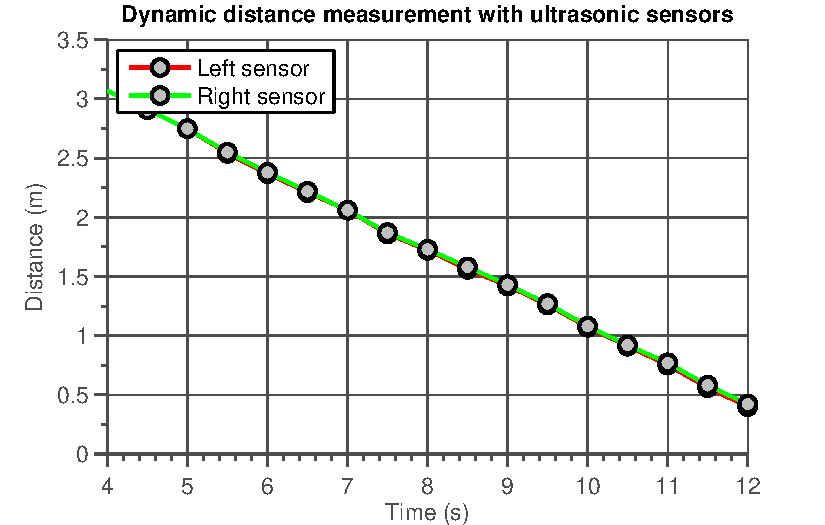
\includegraphics[width=0.6\linewidth]{resource/distance-rc.pdf}
	\end{center}
	\caption{Distances measured in the dynamic measurements}
	\label{fig:ass-2-dyn-dist}
\end{figure}

Using the data graphically illustrated in Figure~\ref{fig:ass-2-dyn-dist}, the velocity and acceleration of KITT can be calculated. This is illustrated in Figure \ref{fig:ass-2-dyn-vel} and \ref{fig:ass-2-dyn-acc}.

\begin{figure}[H]
	\begin{subfigure}{.5\textwidth}
		\begin{center}
			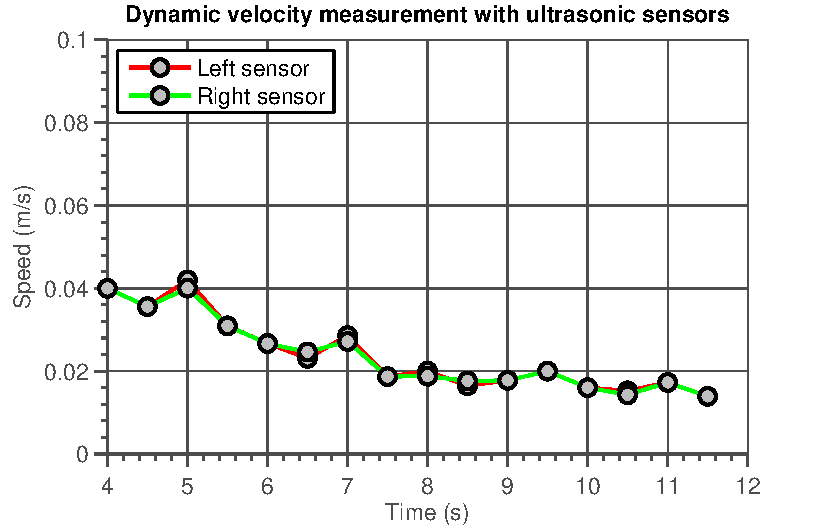
\includegraphics[width=\linewidth]{resource/speed-rc.pdf}
		\end{center}
		\caption{Velocity measured in the dynamic measurements}
		\label{fig:ass-2-dyn-vel}
	\end{subfigure}
	\begin{subfigure}{.5\textwidth}
		\begin{center}
			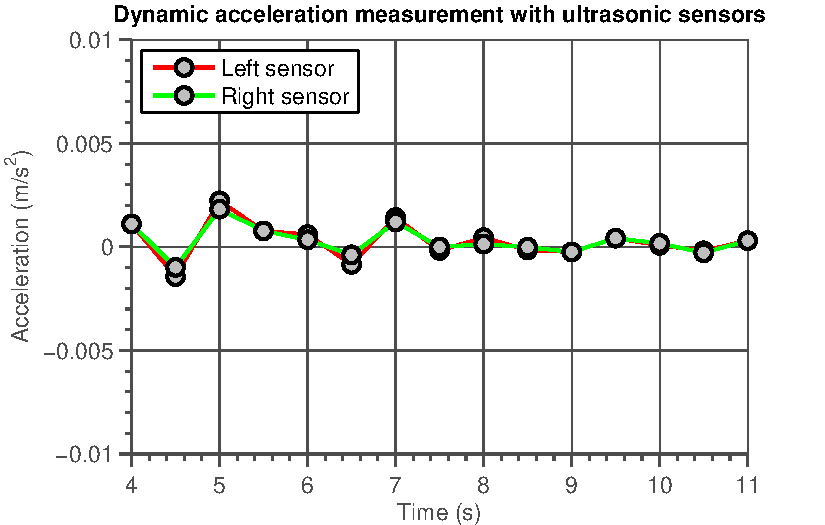
\includegraphics[width=\linewidth]{resource/acceleration-rc.pdf}
		\end{center}
		\caption{Acceleration measured in the dynamic measurements}
		\label{fig:ass-2-dyn-acc}
	\end{subfigure}
	\caption{Velocity and acceleration results of the dynamic measurements}
\end{figure}

Figure \ref{fig:ass-2-dyn-dist} shows that time and distance are approximately linearily related, which would indicate a near constant velocity. This agrees with our experiment, as we programmed KITT to drive at a constant velocity. However, Figure \ref{eq:ass-2-vel-car} shows a somewhat fluctuating speed which decreases with time. This is due to the decrease of the battery voltage and the low speed of KITT. We programmed KITT to drive at a minimal speed, in order to obtain the most information. However, at such a low speed, KITT's motors did just not supply enough torque to maintain this speed. At last, the average acceleration is zero. This resembles our expectancy, as a constant duty cycle of the PWM signal of the motor produces a constant torque.

\section{Signal filtering}
bla

\section{Datasheet}
We filled out the blank field in KITT's datasheet as depicted in Table \ref{tab:ass2-datasheet}.

\begin{table}[H]
	\centering
	\caption{Blank fields of KITT's datasheet}
	\label{tab:ass2-datasheet}
	\begin{tabular}{c c}
		\hline\hline
		Field & Value \\
		\hline
		Bluetooth operating frequency & \SI{2.4}{GHz} to \SI{2.485}{GHz} \\
		Bluetooth operating range & 24 m
		\hline
		\end{tabular}
\end{table}

\end{document}